\documentclass[a4paper,11pt,fleqn]{scrartcl}%fleqn pour aligner les equations à gauche
\usepackage{../../Styles/Exercice}


\newcommand{\chnum}{Chapitre 14}
\newcommand{\chtitle}{Modélisation de l'écoulement d'un fluide}
\newcommand{\dtype}{Exercices}
  
\begin{document}
	\maketitle
\begin{multicols}{2}
\section{Comprendre le déplacement vertical des poissons}
Pour se déplacer verticalement, les poissons utilisent leurs vessie natatoire : il s'agit d'une poche plus ou moins remplie de gaz. C'est elle qui détermine la profondeur à laquelle le poisson flotte dans l'eau.
\begin{enumerate}
	\item Citer la grandeur physique qui varie quand un poisson gonfle ou dégonfle sa vessie natatoire.
	\item Établir le bilan des forces s'exerçant sur un poisson immobile à la profondeur $h$ et prédire le sens du mouvement si le poisson gonfle sa vessie natatoire.
\end{enumerate}

\section{Calculer une norme}
Une barque flotte grâce à la poussée d'Archimère.
\begin{enumerate}
	\item Calculer la norme de la poussée d'Archimède qui s'exerce sur la barque dont la partie immergée a un volume $V=\SI{2,0}{\meter\cubed}$.
	\item Expliquer qualitativement l'origine de la poussée d'Archimède.
\end{enumerate}

\section{Calculer un débit volumique}
Un robinet ouvert laisse couler \SI{1,5}{L} d'eau par minute. L'aire de la section du jet en sortie de robinet vaut $S=\SI{1,0}{\centi\meter\squared}$.
\begin{enumerate}
	\item Exprimer puis calculer le débit volumique du jet.
	\item Exprimer puis calculer la vitesse d'écoulement de l'eau en sortie du robinet.
\end{enumerate}

\section{Calculer une dépression}
Un écoulement  horizontal d'air est initialement à la vitesse $v_1=\SI{5,0}{\meter\per\second}$ dans une section droite de conduit d'aire $S_1=\SI{2,0}{\centi\meter\squared}$. Suite à un étranglement, la section droite de la seconde partie du conduit a une aire $S_2=\SI{1,0}{\centi\meter\squared}$.\\
\textbf{Donnée :} $\rho_{air} =\SI{1,2}{\kilo\gram\per\meter\cubed}$
\begin{enumerate}
	\item Exprimer puis calculer la vitesse $v_2$ de l'écoulement de l'air dans la seconde partie du circuit.
	\item Exprimer puis calculer la dépression $P_1-P_2$ résultant de ce changement de section?
\end{enumerate}

\section{Calculer une vitesse d'éjection de vidange}
La vidange d'un réservoir d'eau est représenté ci-après. La section de l'ouverture de vidange $s$ est très petite devant la surface libre $S$ du liquide, ce qui permet en première approximation de supposer la surface libre du liquide immobile.
\begin{itemize}
	\item Exprimer puis calculer la vitesse d'écoulement du liquide par la section $s$ pour $h_0=\SI{1,0}{m}$.
\end{itemize}
\begin{center}
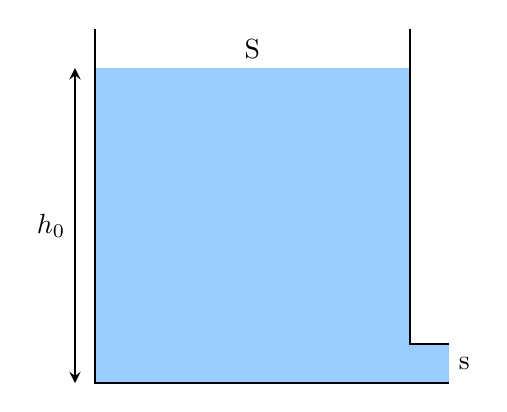
\begin{tikzpicture}
\definecolor{mycolor}{RGB}{153,204,255}
	\fill[mycolor] (0,0) rectangle (4,4);
	\fill[mycolor] (4,0) rectangle (4.5,0.5);
	\draw[thick] (0,4.5)--(0,0)--(4.5,0);
	\draw[thick] (4,4.5)--(4,0.5)--(4.5,0.5);
	\node[above] (S) at (2,4){S}; 
	\node[right] (s) at (4.5,.25){s};
	\node[left] (h) at (-.25,2){$h_0$};
	\draw[stealth-stealth,thick] (-.25,0) to (-.25,4); 
\end{tikzpicture}
\end{center}


\section{Siphon}
Pour vider partiellement un réservoir parallélépipédique contenant de l'eau, on utilise un siphon qui est un tube de section d'aire constante $s$. On note $\Sigma$ l'aire de la section du réservoir. Soient $A$ le point d'entrée du siphon, $B$ le point le plus haut du siphon, $C$ un point à la sortie du siphon et $D$ un point de la surface libre dans le réservoir? la surface libre dans le réservoir et l'extrémité $C$ du siphon sont à la pression atmosphérique $P_a$. L'origine des ordonnées est au fond du réservoir.\\
\textbf{Données :}
\begin{itemize}
	\item $z_A=\SI{5,0}{cm}$ ; $z_B=\SI{70}{cm}$ ;$z_C=\SI{-10}{cm}$ ; à l'instant initial : $z_D=\SI{60}{cm}$.
	\item $\Sigma= \SI{1,0}{\meter\squared}$
	\item $s=\SI{1,0}{\centi\meter\squared}$   
\end{itemize}
\begin{enumerate}
	\item En considérant que $s<<\Sigma$, comparer les vitesses d'écoulement de l'eau au point $D$ et au point $C$.
	\item Calculer la vitesse d'écoulement de l'eau à la sortie du siphon. En déduire un condition pour que le fluide s'écoule.
	\item Calculer les pressions $P_A$ et $P_B$ dans l'eau aux points $A$ et $B$.
	\item En déduire ce qu'il faut faire pour amorcer le siphon? La hauteur du point $B$ peut-elle être quelconque ?
\end{enumerate}
\begin{center}
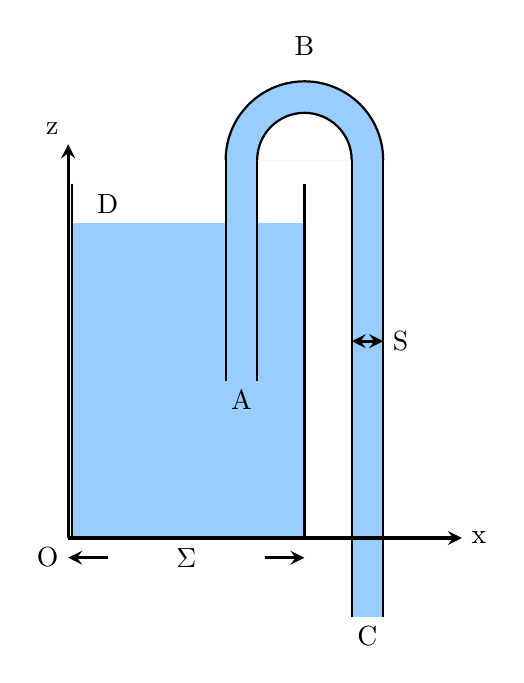
\begin{tikzpicture}
\definecolor{mycolor}{RGB}{153,204,255}

	\fill[mycolor] (0.05,0) rectangle (3,4);
	\fill[mycolor] (2,4) rectangle(2.4,5);
	\fill[mycolor] (3.6,-1) rectangle(4,4.8);
	
	\draw[-stealth,very thick] (0,0) to (0,5);
	\draw[-stealth,very thick] (0,0) to (5,0);
	\draw[thick] (0.05,4.5) -- (0.05,0) --(3,0) --(3,4.5);
	\draw[thick] (2,2)--(2,4.8);
	\draw[thick] (2.4,2)--(2.4,4.8);
	\draw[thick,fill=mycolor] (2,4.8) arc(180:0:1);
	\draw[thick,fill=white] (2.4,4.8) arc(180:0:.6);
	
	\draw[thick] (4,-1)--(4,4.8);
	\draw[thick] (3.6,-1)--(3.6,4.8);
	
	\node[above left] (z) at (0,5){z};
	\node[below left] (O) at (0,0){O};
	\node[above] (D) at (.5,4){D};
	\node[below] (A) at (2.2,2){A};
	\node[above] (B) at (3,6){B};
	\node[below] (C) at (3.8,-1){C};
	\node[right] (x) at (5,0){x};
	
	\node (Sigma) at (1.5,-.25){$\Sigma$};
	\node[right] (S) at (4,2.5){S};
	
	\draw[stealth-,very thick] (0,-.25) to (.5,-.25);
	\draw[-stealth,very thick] (2.5,-.25) to (3,-.25);
	\draw[stealth-stealth,very thick] (3.6,2.5) to (4,2.5);
	
	
\end{tikzpicture}
\end{center}
\end{multicols}
\end{document}

\section{Tube de Venturi}
Sur un tube de Venturi, un tube en U contenant du mercure \ce{Hg} est branché entre deux positions 1 et 2. De l'eau traverse le tube avec un débit volumique $D_V$. Dans la direction perpendiculaire à l'écoulement horizontal de l'eau dans le tube, les fluides sont statiques.
\begin{center}
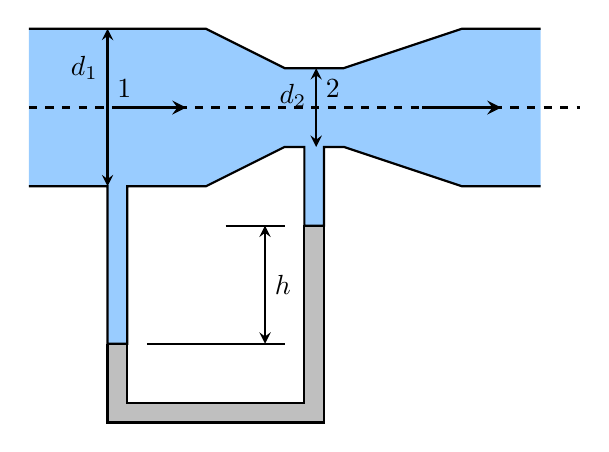
\begin{tikzpicture}
\definecolor{mycolor}{RGB}{153,204,255}

	\fill[mycolor] (0,0)--(1,0)--(1,-2)--(1.25,-2)--(1.25,0) -- (2.25,0) --(3.25,.5)--(3.5,.5)--(3.5,-.5)--(3.75,-.5)--(3.75,.5)--(4,.5)--(5.5,0)--(6.5,0)--(6.5,2)--(5.5,2)--(4,1.5)--(3.25,1.5)--(2.25,2)--(0,2)--cycle;
	\fill[gray!50] (1,-2)--(1,-3)--(3.75,-3)--(3.75,-.5)--(3.5,-.5)--(3.5,-2.75)--(1.25,-2.75)--(1.25,-2) --cycle;
	\draw[thick] (0,0)--(1,0)--(1,-2)--(1.25,-2)--(1.25,0) -- (2.25,0) --(3.25,.5)--(3.5,.5)--(3.5,-.5)--(3.75,-.5)--(3.75,.5)--(4,.5)--(5.5,0)--(6.5,0);
	\draw[thick] (6.5,2)--(5.5,2)--(4,1.5)--(3.25,1.5)--(2.25,2)--(0,2);
	\draw[thick] (1,-2)--(1,-3)--(3.75,-3)--(3.75,-.5)--(3.5,-.5)--(3.5,-2.75)--(1.25,-2.75)--(1.25,-2);
	
	\draw[dashed,thick] (0,1) --(7,1);
	\draw[-stealth,very thick] (1.1,1) to (2,1);
	\draw[stealth-stealth,thick] (1,0) to (1,2);
	\node[above right] at (1,1){1};
	\node[left] (d1) at (1,1.5){$d_1$};
	
	\draw[stealth-stealth,thick] (3.65,.5) to (3.65,1.5);
	\node[above right] at (3.65,1){2};
	\node[left] (d2) at (3.65,1.15){$d_2$};
	
	\draw[-stealth,very thick] (5,1) to (6,1);
	
	\draw[thick] (1.5,-2)--(3.25,-2);
	\draw[thick] (2.5,-.5)--(3.25,-.5);
	\draw[stealth-stealth,thick] (3,-.5) to (3,-2);
	\node[right] (h) at(3,-1.25){$h$};
	
\end{tikzpicture}
\end{center}

\textbf{Données :}
\begin{itemize}
	\item Masses volumiques : $\rho_{\ce{Hg}}=\SI{13550}{\kilo\gram\per\meter\cubed}$ ; $\rho_{eau}=\SI{1000}{\kilo\gram\per\meter\cubed}$.
	\item Diamètres des sections : $d_1=\SI{10}{\milli\meter}$ ; $d_2=\SI{5,0}{\milli\meter}$.
\end{itemize}
\begin{enumerate}
	\item Exprimer puis calculer la différence de pression entre les positions 1 et 2, en fonction de la différence de niveaux $h$, puis en fonction du débit volumique du fluide $D_V$.
	\item Exprimer puis calculer le débit volumique $D_V$ du fluide en fonction de la différence de niveaux$h$ mesurée dans le tube en U.
\end{enumerate}